%!TEX root = ../thesis.tex
%*******************************************************************************
%****************************** Second Chapter *********************************
%*******************************************************************************

\chapter{Methodology}

\ifpdf
    \graphicspath{{Chapter2/Figs/Raster/}{Chapter2/Figs/PDF/}{Chapter2/Figs/}{Chapter2/Figures/}}
\else
    \graphicspath{{Chapter2/Figs/Vector/}{Chapter2/Figs/}{Chapter2/Figures/}}
\fi

\section{PILCO}
PILCO \cite{deisenroth2011pilco} is a model-based indirect policy search method for continuous state $\mathbf{x} \in \mathbb{R}^{D}$ and action $\mathbf{u} \in \mathbb{R}^{F}$ dynamical systems described by
\begin{equation}
    \mathbf{x}_{t+1}=f\left(\mathbf{x}_{t}, \mathbf{u}_{t}\right)+\mathbf{\eta}, \quad \mathbf{\eta} \sim \mathcal{N}\left(\mathbf{0}, \boldgreek{\Sigma}_{\eta}\right)
\end{equation}
where the transition dynamics $f$ of the system are unknown. The objective is to find a deterministic \textit{controller/policy} $\pi : \mathbf{x} \mapsto \pi(\mathbf{x}, \boldgreek{\theta})=\mathbf{u}$ such that the expected return   \cite{deisenroth2013gaussian}
\begin{equation}
    J^{\pi}(\theta)=\sum_{t=0}^{T} \mathbb{E}_{\mathbf{x}_{t}}\left[c\left(\mathbf{x}_{t}\right)\right], \quad \mathbf{x}_{0} \sim \mathcal{N}\left(\boldgreek{\mu}_{0}, \boldgreek{\Sigma}_{0}\right)
    \label{Eq:PILCO-expected-return}
\end{equation}
is minimised after following $\pi$ for $T$ steps. The policy is parametrised by $\mathbf{\theta}$, which take the form of nonlinear RBF networks, where $\mathbf{\theta}$ are the weights and features, or linear-affine transformations, where $\mathbf{\theta}$ are the weights matrix and bias terms. The \textit{cost} $c(\mathbf{x}_{t})$, or negative reward, of being in state $\mathbf{x}$ at time $t$ is the generalised binary saturating cost \cite{deisenroth2013gaussian}
\begin{equation}
    c(\mathbf{x}_{t})=1-\exp \left(-\frac{1}{2 \sigma_{c}^{2}} d\left(\mathbf{x}_{t}, \mathbf{x}_{\text { target }}\right)^{2}\right) \in[0,1]
    \label{Eq:PILCO-cost-function}
\end{equation}
which exclusively penalises the Euclidean distance $d$ from the current state $\mathbf{x}_{t}$ to the target state $\mathbf{x}_{\text { target }}$. $c(\mathbf{x}_{t})$ is locally quadratic and saturates at 1 for large differences between the current state and target state. The saturation distance is controlled by the width parameter $\sigma_{c}$.

\subsection{GP Model Learning}
\label{PILCO:GP-model-learning}
The system dynamics are modelled as a probabilistic Gaussian Process (GP). Tuples of the state and control vectors $\left(\mathbf{x}_{t}, \mathbf{u}_{t}\right)\in \mathbb{R}^{D+F}$ serve as training inputs and differences $\Delta_{t}=\mathbf{x}_{t+1}-\mathbf{x}_{t}+\varepsilon \in \mathbb{R}^{D},\quad \varepsilon \sim \mathcal{N}\left(0, \boldgreek{\Sigma}_{\varepsilon}\right)$ as training targets. Conditionally independent GP's are trained for for each target dimension \cite{deisenroth2010efficient}. The dynamics model provides a \textit{one-step} prediction \cite{deisenroth2011pilco}
\begin{equation}
    p\left(\mathbf{x}_{t+1} | \mathbf{x}_{t}, \mathbf{u}_{t}\right)=\mathcal{N}\left(\mathbf{x}_{t} | \mu_{t}, \boldgreek{\Sigma}_{t}\right)
    \label{Eq:PILCO-one-step-1}
\end{equation}
\begin{equation}
    \mu_{t+1}=\mathbf{x}_{t}+\mathbb{E}_{f}\left[\Delta_{t}\right]
    \label{Eq:PILCO-one-step-2}
\end{equation}
\begin{equation}
    \boldgreek{\Sigma}_{t+1}=\operatorname{var}_{f}\left[\Delta_{t}\right]
    \label{Eq:PILCO-one-step-3}
\end{equation}
where the mean $\mu$ of the state $\mathbf{x}_{t+1}$ is obtained through addition of the current state $\mathbf{x}_{t}$ with the one-step difference prediction $\mathbb{E}_{f}\left[\Delta_{t}\right]$. A GP is defined completely by a mean function $m(\cdot)$ and a positive semidefinite covariance function $K(\cdot,\cdot)$. PILCO follows the common practice of setting the mean prior function to zero and uses the \textit{stationary} anisotropic squared exponential covariance function
\begin{equation}
    k\left(\tilde{\mathbf{x}}_{i}, \tilde{\mathbf{x}}_{j}\right)=\sigma_{0}^{2} \exp \left(-\frac{1}{2}\left(\tilde{\mathbf{x}}_{i}-\tilde{\mathbf{x}}_{j}\right)^{\top} \boldgreek{\Lambda}^{-1}\left(\tilde{\mathbf{x}}_{i}-\tilde{\mathbf{x}}_{j}\right)\right)
    \label{Eq:PILCO-sq-exponential-covariance}
\end{equation}
where $\tilde{\mathbf{x}} = \left[\mathbf{x}\quad\mathbf{u}\right]^{T}$ is the state-action vector, $\boldgreek{\Lambda} =\operatorname{diag}\left(\left[\ell_{1}^{2}, \ldots, \ell_{D+F}^{2}\right]\right)$ depends on the characteristic lengthscales and $\sigma_{0}$ is the variance of the latent function \cite{deisenroth2013gaussian}. The lengthscales determine the speed that the covariance decays with the distance between inputs \cite{quia2010sparse}.

\subsection{Policy Evaluation}
\label{PILCO:policy-evaluation}
PILCO evaluates a given policy by predicting the state evolution over the course of an episode. This is accomplished by propagating uncertain inputs through the dynamics model, using the one-step predictions (Eqs. \ref{Eq:PILCO-one-step-1} - \ref{Eq:PILCO-one-step-3}), to obtain $p\left(\mathbf{x}_{1} | \pi\right), \ldots, p\left(\mathbf{x}_{T} | \pi\right)$ from a given start state distribution $p\left(\mathbf{x}_{0}\right)$. Predicting $\mathbf{x}_{t+1}$ from $p(\mathbf{x}_{t})$ requires evaluation of the predictive distribution over state differences
\begin{equation}
    p\left(\Delta_{t}\right)=\iint p\left(f\left(\tilde{\mathbf{x}}_{t}\right) | \left(\tilde{\mathbf{x}}_{t}\right)\right) p\left(\tilde{\mathbf{x}}_{t}\right) \mathrm{d} f \mathrm{d} \tilde{\mathbf{x}}_{t},
    \label{Eq:PILCO-predictive-state-differences}
\end{equation}
by integrating out the random function of the GP distribution and the random variable $\tilde{\mathbf{x}}_{t}$. Here $p\left(\tilde{\mathbf{x}}_{t}\right)=p\left(\mathbf{x}_{t}, \mathbf{u}_{t}\right)$ is the joint state-action distribution. Since the predictive distribution in Eq. \ref{Eq:PILCO-predictive-state-differences} is analytically intractable for uncertain inputs, it is approximated as a Gaussian distribution using \textit{moment matching} (see Fig. \ref{Fig:moment-matching}). This approximation ensures that the state distribution is given by $p\left(\tilde{\mathbf{x}}_{t}\right)=\mathcal{N}\left(\tilde{\mathbf{x}}_{t} | \tilde{\mathbf{\mu}}_{t}, \tilde{\boldgreek{\Sigma}}_{t}\right)$ for all $t$. This, alongside the choice of cost function (Eq. \ref{Eq:PILCO-cost-function}) enables the expected return (Eq. \ref{Eq:PILCO-expected-return}) to be evaluated analytically according to
\begin{equation}
    \mathbb{E}_{\mathbf{x}_{t}}\left[c\left(\mathbf{x}_{t}\right)\right]=\int c\left(\mathbf{x}_{t}\right) \mathcal{N}\left(\mathbf{x}_{t} | \boldgreek{\mu}_{t}, \boldgreek{\Sigma}_{t}\right) \mathrm{d} \mathbf{x}_{t}
\end{equation}
for $t=1,\dots,T$.

\begin{figure}
\centering    
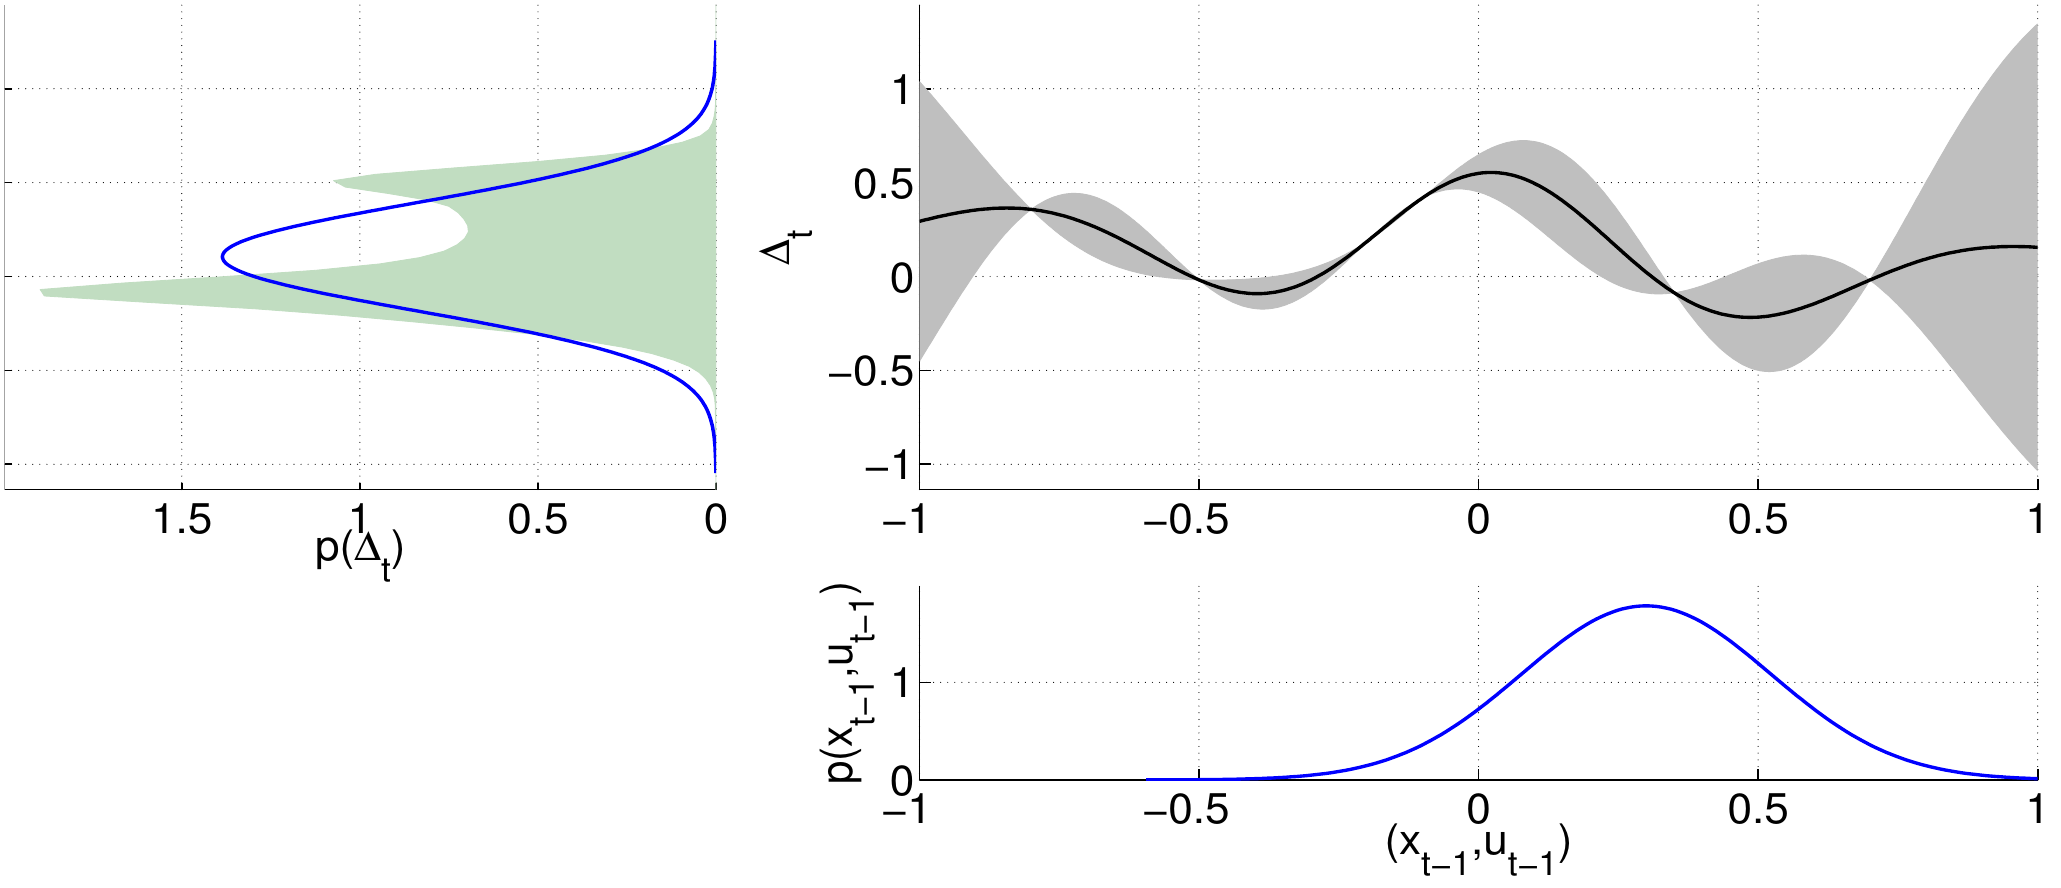
\includegraphics[width=1.0\textwidth]{PILCO-moment-matching.png}
\caption[Propagating an uncertain input through the GP dynamics model]{Propagating an uncertain input through the GP dynamics model (upper right panel). The input distribution $p(x_{t-1},u_{t-1})$, assumed to be Gaussian (lower right panel), is propagated through the dynamics model yielding the shaded distribution $p(\Delta_{t})$. The shaded distribution is then approximated by a Gaussian with the same mean and variance (upper left panel). Reproduced from \cite{deisenroth2011pilco}.}
\label{Fig:moment-matching}
\end{figure}

\subsection{Policy Improvement}
\label{PILCO:policy-improvement}
PILCO is an indirect policy search method and does not require an explicit value function model. Instead it learns a \textit{parametrised policy} that can select actions without consulting a value function. Due to the moment matching approximation, the state distribution is considered to be Gaussian $p\left(\tilde{\mathbf{x}}_{t}\right)=\mathcal{N}\left(\tilde{\mathbf{x}}_{t} | \tilde{\mathbf{\mu}}_{t}, \tilde{\boldgreek{\Sigma}}_{t}\right)$ for all $t$, where $\tilde{\mathbf{x}}_{t} = (\mathbf{x}_{t},\mathbf{u}_{t})$. The control signal  $\mathbf{u}_{t-1} = \pi\left(\mathbf{x}_{t-1}, \theta\right)$ is a function of the state, and hence the next state is also functionally dependent on the mean $\mu_{u}$ and covariance $\boldgreek{\Sigma}_{u}$ of the control signal. This relationship allows the gradients of the expected return $J^{\pi}$, with respect to the policy parameters $\boldgreek{\theta}$, to be computed analytically. The policy parameters are then learned to \textit{maximise} performance (\textit{minimise} cost) for a given task, so their updates approximate gradient \textit{descent} in $J$ \cite{sutton2018reinforcement}:
\begin{equation}
    \boldgreek{\theta}_{t+1}=\boldgreek{\theta}_{t} - \alpha\nabla J^{\pi}\left(\boldgreek{\theta_{t}}\right),
\end{equation}
where $\alpha$ is the learning rate. For a more thorough explanation of PILCO see \cite{deisenroth2011pilco}\cite{deisenroth2010efficient}\cite{deisenroth2013gaussian}. Algorithm \ref{PILCO:algorithm-1} provides an overview of PILCO.

\begin{algorithm}
\caption{PILCO}\label{PILCO:algorithm-1}
\begin{algorithmic}[1]
\State \textbf{init:} Sample controller parameters $\boldgreek{\theta} \sim \mathcal{N}\left(\mathbf{0},\mathbf{I}\right)$
\Repeat{}
\State Learn probabilistic GP dynamics model using all environment data \Comment{Sec \ref{PILCO:GP-model-learning}}
\Repeat{}
\State Approximate inference for policy evaluation: $J^{\pi}\left(\theta\right)$ \Comment{Sec \ref{PILCO:policy-evaluation}}
\State Gradient-based policy improvement: $\mathrm{d} J^{\pi}(\boldsymbol{\theta}) / \mathrm{d} \boldsymbol{\theta}$ \Comment{Sec \ref{PILCO:policy-improvement}}
\State Update parameters $\boldgreek{\theta}$\Comment{CG or L-BFGS}
\Until convergence; \textbf{return} $\boldgreek{\theta}^{*}$
\State Set $\pi^{*} \gets \pi\left(\theta^{*}\right)$
\State  Apply $\pi^{*}$ to environment and record data
\Until task learned \Comment{modified from \cite{deisenroth2011pilco}}
\end{algorithmic}
\end{algorithm}

\section{Approximating PILCO's GP}
At the heart of the Monte Carlo uncertainty approximation is the need for one-step predictions using a function sampled from the posterior distribution of PILCO's dynamics model. The use of the squared exponential covariance function in PILCO's GP corresponds to a Bayesian linear regression model with an infinite number of basis functions \cite{williams2006gaussian}. This means drawing a representative function requires an infinite number of weights since each basis function is accompanied by its own weight. To overcome this issue, a finite-weight stationary trigonometric Bayesian regression model \cite{quia2010sparse} is used to approximate PILCO's GP. In addition to solving the sampling issue, this model provides other advantages. First, the periodicity of the trigonometric basis functions means that one does not need to explicitly specify the mean for each basis function. Second, a direct GP implementation has practical limitations with regards to computational and memory requirements, which scale as $\mathcal{O}(n^{2})$ and $\mathcal{O}(n^{3})$, respectively. The trigonometric model has computational requirements of $\mathcal{O}(nm^{2})$ and memory requirements of $\mathcal{O}(nm)$ where $m<<n$ \cite{quia2010sparse}, which are typical values for sparse GP approximations \cite{quinonero2005unifying}. The largest PILCO environment used for this research (cart double pendulum) generates approximately $4k$ data points. The model is first introduced here in a traditional treatment of Bayesian linear regression. Section \ref{S:one-step-predictions} relates the model to PILCO's one-step predictions. Finally, section \ref{S:sparse-approximation} shows that the model can be viewed as a sparse stationary GP that can approximate any full GP.

The model consists of a linear combination of trigonometric functions \cite{quia2010sparse}
\begin{equation}
    f(\mathbf{x})=\sum_{r=1}^{m} a_{r} \cos \left(2 \pi \mathbf{s}_{r}^{\top} \mathbf{x}\right)+b_{r} \sin \left(2 \pi \mathbf{s}_{r}^{\top} \mathbf{x}\right)
    \label{Eq:Model-trigonometric-model}
\end{equation}
where $\mathbf{s}_{r}$ is a $D$-dimensional vector of spectral frequencies shared by each pair of basis functions while $a_{r}$ and $b_{r}$ are amplitude parameters which are independent for each basis function (see Sec \ref{S:sparse-approximation} for selecting spectral frequencies). The amplitudes have independent Gaussian priors with linearly scaled variances 
\begin{equation}
    a_{r} \sim \mathcal{N}\left(0, \frac{\sigma_{0}^{2}}{m}\right), \quad b_{r} \sim \mathcal{N}\left(0, \frac{\sigma_{0}^{2}}{m}\right)
\end{equation}
where $m$ are the number basis functions. The frequencies function as deterministic parameters and the amplitudes are treated in a Bayesian fashion. For this, the model is packaged as the dot product between the set of amplitudes and the basis functions 
\begin{equation}
    f(\mathbf{x}, \mathbf{w}) = \mathbf{w}^{\top} \varphi\left(\mathbf{x}\right)
\end{equation}
where $\mathbf{x}$ is a $D$-dimensional input variable, $\mathbf{w}=\left[a_{1}, b_{1}, \dots, a_{m}, b_{m}\right]^{\top}$ are the model weights and
\begin{equation}
    \varphi(\mathbf{x})=\left[\cos \left(2 \pi \mathbf{s}_{1}^{\top} \mathbf{x}\right)\quad \sin \left(2 \pi \mathbf{s}_{1}^{\top} \mathbf{x}\right) \quad\ldots\quad \cos \left(2 \pi \mathbf{s}_{m}^{\top} \mathbf{x}\right) \quad \sin \left(2 \pi \mathbf{s}_{m}^{\top} \mathbf{x}\right)\right]^{\top}.
\end{equation}
The model targets are now assumed to have been generated by the function $f(\mathbf{x}, \mathbf{w})$ and independently corrupted by additive Gaussian noise of constant variance $\sigma_{n}^{2}$
\begin{equation}
    y = f(\mathbf{x}, \mathbf{w}) + \varepsilon, \quad \varepsilon \sim \mathcal{N}\left(0,\sigma_{n}^{2}\right).
\end{equation}
This can be written as 
\begin{equation}
    p(y | \mathbf{x}, \mathbf{w}, \sigma^{2}_{n})= \mathcal{N}\left(y | f(\mathbf{x}, \mathbf{w}), \sigma^{2}_{n}\right).
    \label{Eq:Model-one-value-likelihood}
\end{equation}
For a dataset of model inputs $\mathbf{X}=\left\{\mathbf{x}_{1}, \dots, \mathbf{x}_{N}\right\}$ with corresponding target values $\mathbf{y}=\{y_{1}, \dots, y_{N}\}$ and assuming that these data points have been drawn independently from $\mathcal{N}(y|f(\mathbf{x}, \mathbf{w}), \sigma^{2}_{n})$, the likelihood function is
\begin{equation}
    p(\mathbf{y} | \mathbf{X}, \mathbf{w}, \sigma^{2}_{n})=\prod_{i=1}^{N} \mathcal{N}\left(y_{i} | \mathbf{w}^{\top} \varphi\left(\mathbf{x}_{i}\right), \sigma^{2}_{n}\right).
\end{equation}
The posterior distribution over the model weights is proportional to the product of the likelihood function and the prior. Since the Gaussian prior is conjugate, the posterior distribution is also Gaussian (see Appendix \ref{A:derivation-posterior-over-weights} for derivation)
\begin{equation}
    q(\mathbf{w} | \mathbf{y}, \mathbf{X}, \sigma_{0}^{2}, \sigma_{n}^{2})=\mathcal{N}\left(\mathbf{w} | \mathbf{\mu_{\mathbf{w}}}, \mathbf{A}^{-1}\right)
    \label{Eq:Model-posterior-over-weights}
\end{equation}
where the posterior mean $\mu_{\mathbf{w}}$ and precision matrix $A$ are
\begin{equation}
    \mathbf{\mu_{\mathbf{w}}}=\frac{1}{\sigma_{n}^{2}} \mathbf{A}^{-1} \Phi \mathbf{y}
\end{equation}
\begin{equation}
    \mathbf{A} =\frac{1}{\sigma_{n}^{2}} \Phi \Phi^{\top} + \frac{m}{\sigma_{0}^{2}} \mathbf{I}_{2m}.
\end{equation}
Here, $\Phi = \left[\varphi(\mathbf{x}_{1}), \dots , \varphi(\mathbf{x}_{N})\right]$ is the $2m$ by $N$ \textit{design matrix}.

To make a prediction $y_{*}$ for a new input value $\textbf{x}_{*}$ requires evaluation of the predictive distribution, defined by
\begin{equation}
   p(y_{*} | \mathbf{y},\mathbf{X},\mathbf{x}_{*}, \sigma_{0}^{2}, \sigma_{n}^{2})=\int p(y_{*} | \mathbf{x}_{*}, \mathbf{w}, \sigma_{n}^{2}) q(\mathbf{w} | \mathbf{y}, \mathbf{X}, \sigma_{0}^{2}, \sigma_{n}^{2}) \mathrm{d} \mathbf{w}
\end{equation}
where the conditional distribution of the target variable $p(y_{*} | \mathbf{x}_{*}, \mathbf{w}, \sigma_{n}^{2})$ is defined by Eq. \ref{Eq:Model-one-value-likelihood} and the posterior distribution over the weights is given by Eq. \ref{Eq:Model-posterior-over-weights}. The predictive distribution for a single input is (see Appendix \ref{A:derivation-predictive-distribution} for derivation)
\begin{equation}
    p(y_{*} | \mathbf{y},\mathbf{X},\mathbf{x}_{*}, \sigma_{0}^{2}, \sigma_{n}^{2}) = \mathcal{N}\left(y_{*} | \mathbf{\mu}_{y_{*}}, \sigma_{y_{*}}^{2}\right)
    \label{Eq:Model-predicitive-distribution}
\end{equation}
where
\begin{equation}
    \mu_{y_{*}} = \frac{1}{\sigma_{n}^{2}}\varphi(\mathbf{x}_{*})^{\top} \mathbf{A}^{-1} \Phi \mathbf{y}
\end{equation}
\begin{equation}
    \sigma_{y_{*}}^{2}=\sigma_{n}^{2} + \varphi(\mathbf{x}_{*})^{\top}\mathbf{A}^{-1}\varphi(\mathbf{x}_{*}).
    \label{Eq:Model-predictive-variance}
\end{equation}
\paragraph{A note on model uncertainty:} The predictive variance (Eq. \ref{Eq:Model-predictive-variance}) consists of two terms. The first represents the noise present on the data while the second quantifies the uncertainty associated with the model weights $\textbf{w}$ \cite{bishop2006pattern}. The latter is particularly relevant to this research and will be expanded on in Section \ref{S:disentangling-uncertainty}. As more data is observed, the model becomes increasingly confident and consequently the posterior distribution narrows due to contraction of the second term. \citet{qazaz1997upper} show that $\sigma_{y_{*}(N+1)}^{2} \leqslant \sigma_{y_{*}(N)}^{2}$ while in the limit $N \to \infty$ the second term of Eq. \ref{Eq:Model-predictive-variance} reduces to zero. In this case the model has full confidence in the weights and the predictive variance's sole contributor is the data noise governed by the $\sigma_{n}^2$ term.

\subsection{One-Step Predictions}
\label{S:one-step-predictions}
The trigonometric basis function model used to approximate PILCO's GP is also trained with tuples of the state and control vectors $\tilde{\mathbf{x}}_{t}=\left(\mathbf{x}_{t}, \mathbf{u}_{t}\right)\in \mathbb{R}^{D+F}$ as training inputs and state differences $\Delta_{t}=\mathbf{x}_{t+1}-\mathbf{x}_{t}+\varepsilon,\quad \varepsilon \sim \mathcal{N}\left(0, \boldgreek{\Sigma}_{\varepsilon}\right)$ as targets. However, while the one-step predictions generated by PILCO's GP dynamics model are produced by the posterior predictive distribution, for the uncertainty estimations in Sec \ref{S:disentangling-uncertainty}, functions drawn from the posterior distribution over the model weights are used to make one-step predictions. For this, first a set of $2m$ weights is drawn from the posterior distribution $\mathbf{w} \sim q(\mathbf{w})$ (Eq. \ref{Eq:Model-posterior-over-weights}) where the conditioning variables are dropped for brevity. The one-step predictions are then computed with
\begin{equation}
    \mathbf{x}_{t+1}
    = \mathbf{x}_{t} + \Delta_{t} \\
    =\mathbf{x}_{t}+\mathbf{w}^{\top}\varphi(\tilde{\mathbf{x}}_{t}).
    \label{Eq:model-posterior-one-step}
\end{equation}

\subsection{A Sparse Approximation to the Full GP}
\label{S:sparse-approximation}
This section follows the treatment in \cite{quia2010sparse} and relates the trigonometric basis function model of the previous section to a full GP by creating a sparse representation of the stationary covariance function. GP regression is a probabilistic, non-parametric Bayesian approach that is completely specified by a mean function and covariance function \cite{williams2006gaussian}
\begin{equation}
    \begin{aligned} 
    m(\mathbf{x}) 
    &=\mathbb{E}[f(\mathbf{x})] \\ k\left(\mathbf{x}_{i}, \mathbf{x}_{j}\right) &=\mathbb{E}\left[(f(\mathbf{x}_{i})-m(\mathbf{x}_{i}))\left(f\left(\mathbf{x}_{j}\right)-m\left(\mathbf{x}_{j}\right)\right)\right]. 
    \end{aligned}
\end{equation}
Similar to the PILCO GP, a zero mean function $m(\mathbf{x})=0$ and stationary squared exponential covariance function
\begin{equation}
    k\left(\mathbf{x}_{i}, \mathbf{x}_{j}\right)=k\left(\mathbf{x}_{i}-\mathbf{x}_{j}\right)=k(\tau)
    \label{Eq:stationary-covariance-tau}
\end{equation}
are considered (see Eq \ref{Eq:PILCO-sq-exponential-covariance}). A stationary covariance function is a function $\boldgreek{\tau} = \mathbf{x}_{i}-\mathbf{x}_{j}$ that depends only on the difference between inputs. Now considering the trigonometric basis function model in Eq \ref{Eq:Model-trigonometric-model}. Under the prior, the distribution over functions is Gaussian with zero mean and stationary covariance function \cite{quia2010sparse}
\begin{equation}
    k\left(\mathbf{x}_{i}, \mathbf{x}_{j}\right)=\frac{\sigma_{0}^{2}}{m} \varphi\left(\mathbf{x}_{i}\right)^{\top} \varphi\left(\mathbf{x}_{j}\right)=\frac{\sigma_{0}^{2}}{m} \sum_{r=1}^{m} \cos \left(2 \pi \mathbf{s}_{r}^{\top}\left(\mathbf{x}_{i}-\mathbf{x}_{j}\right)\right).
    \label{Eq:phi-to-covariance-relationship}
\end{equation}
\begin{theorem}[Bochner's theorem]
\label{T:bochners-theorem}
A complex-valued function $k$ on $\mathbb{R}^{D}$ is the
covariance function of a weakly stationary mean square continuous complex-valued random process on $\mathbb{R}^{D}$ if and only if it can be represented as
\begin{equation}
    k(\boldgreek{\tau})=\int_{\mathbb{R}^{D}} e^{2 \pi i \mathbf{s} \cdot \boldgreek{\tau}} d \mu_{fm}(\mathbf{s})
\end{equation}
where $\mu_{fm}$ is a positive finite measure. \Comment{Quoted from \cite{stein1999interpolation}}
\end{theorem}
If $\mu_{fm}$ has a probability density $S(\mathbf{s})$ then $S$ is the \textit{spectral density} associated with $k$ \cite{williams2006gaussian} and is proportional to a probability measure $S(\mathbf{s}) \propto p_{S}(\mathbf{s})$. The proportionality constant can be obtained by evaluating the covariance function in Eq \ref{Eq:stationary-covariance-tau} at $\boldgreek{\tau}=\mathbf{0}$ to give 
\begin{equation}
    S(\mathbf{s})=k(\mathbf{0}) p_{S}(\mathbf{s})=\sigma_{0}^{2} p_{S}(\mathbf{s}).
\end{equation}
Should $S(\mathbf{s})$ exist, according to the Wiener-Khintchine theorem \cite{chatfield1989timeseries}, the covariance function and the spectral density form a Fourier pair
\begin{equation}
    k(\boldgreek{\tau})=\int S(\mathbf{s}) e^{2 \pi i \mathbf{s} \cdot \boldgreek{\tau}} d \mathbf{s}, \quad S(\mathbf{s})=\int k(\boldgreek{\tau}) e^{-2 \pi i \mathbf{s} \cdot \tau} d \boldgreek{\tau}.
\end{equation}
Since $S(\mathbf{s})$ is proportional to a multivariate probability density in $\mathbf{s}$ the covariance function can be rewritten as an expectation with respect to the probability measure $p_{S}(\mathbf{s})$ 
\begin{equation}
    \begin{aligned}
    k(\boldgreek{\tau})
    &=\int_{\mathbb{R}^{D}} e^{2 \pi i \mathbf{s}^{\top}\left(\mathbf{x}_{i}-\mathbf{x}_{j}\right)} S(\mathbf{s}) \mathrm{d} \mathbf{s}\\
    &=\sigma_{0}^{2} \int_{\mathbb{R}^{D}} e^{2 \pi i \mathbf{s}^{\top} \mathbf{x}_{i}}\left(e^{2 \pi i \mathbf{s}^{\top} \mathbf{x}_{j}}\right)^{*} p_{S}(\mathbf{s}) d \mathbf{s} \\ 
    &=\sigma_{0}^{2} \mathbb{E}_{p_{S}(\mathbf{s})}\left[e^{2 \pi i \mathbf{s}^{\top} \mathbf{x}_{i}}\left(e^{2 \pi i \mathbf{s}^{\top} \mathbf{x}_{j}}\right)^{*}\right] \end{aligned}
    \label{Eq:k-tau-expectation-wrt-ps}
\end{equation}
where the superscript asterisk denotes complex conjugation. The result in Eq. \ref{Eq:k-tau-expectation-wrt-ps} can be estimated by simple Monte Carlo. Since the spectral density is symmetric about zero, sampling frequency pairs $\{\mathbf{s}_{r},-\mathbf{s}_{r}\}$ preserves the exact expansion where the imaginary terms cancel
\begin{equation}
    \begin{aligned} 
    k\left(\mathbf{x}_{i}, \mathbf{x}_{j}\right) 
    & \simeq \frac{\sigma_{0}^{2}}{2 m} \sum_{r=1}^{m}\left[e^{2 \pi i \mathbf{s}_{r}^{\top} \mathbf{x}_{i}}\left(e^{2 \pi i \mathbf{s}_{r}^{\top} \mathbf{x}_{j}}\right)^{*}+\left(e^{2 \pi i \mathbf{s}_{r}^{\top} \mathbf{x}_{i}}\right)^{*} e^{2 \pi i \mathbf{s}_{r}^{\top} \mathbf{x}_{j}}\right] \\ &=\frac{\sigma_{0}^{2}}{m} \operatorname{Re}\left[\sum_{r=1}^{m} e^{2 \pi i \mathbf{s}_{r}^{\top} \mathbf{x}_{i}}\left(e^{2 \pi i \mathbf{s}_{r}^{\top} \mathbf{x}_{j}}\right)^{*}\right] \\
    &=\frac{\sigma_{0}^{2}}{m} \sum_{r=1}^{m} \cos \left(2 \pi \mathbf{s}_{r}^{\top}\left(\mathbf{x}_{i}-\mathbf{x}_{j}\right)\right).
    \end{aligned}
\end{equation}
Here, $Re$ is the real part of the complex number and the finite set of Monte Carlo frequencies $\mathbf{s}_{r}$, called \textit{spectral points}, are sampled from $p_{S}(\mathbf{s})$. This result shows that Eq. \ref{Eq:phi-to-covariance-relationship} is recovered by sparsifying the stationary covariance function of a full GP meaning that the trigonometric basis function model of the previous section is indeed a sparse spectrum Gaussian process. 

Taking the Fourier transform of the squared exponential covariance function used in PILCO's GP dynamics model gives a probability density of multivariate Gaussian form
\begin{equation}
    p_{S}(\mathbf{s})=\frac{1}{k(\mathbf{0})} \int_{\mathbb{R}^{D}} e^{-2 \pi i \mathbf{s}^{\top} \tau} k(\mathbf{\tau}) d \tau=\sqrt{|2 \pi \Lambda|} \exp \left(-2 \pi^{2} \mathbf{s}^{\top} \Lambda \mathbf{s}\right)
    \label{Eq:Gaussian-spectral-points-sample}
\end{equation}
from which the spectral points are drawn for the Monte Carlo estimate of $k(\mathbf{x}_{i},\mathbf{x}_{j})$. 

\subsection{Hyperparameter Optimisation}
In a fully Bayesian treatment of the trigonometric basis function model one would introduce priors over $\sigma_{0}^2$ and $\sigma_{n}^2$ and marginalise with respect to both the hyperparameters and the weights $\mathbf{w}$ to make predictions. However, while marginalisation over either the hyperparameters or the weights is plausible, complete marginalisation over both is analytically intractable \cite{bishop2006pattern}. Instead, here the hyperparameters are learned through optimising the log marginal likelihood (see Appendix ?? for derivation)
\begin{equation}
    \log p\left(\mathbf{y}|\boldgreek{\theta}\right) = -\frac{1}{2\sigma_{n}^{2}}\left[\mathbf{y}^{\top}\mathbf{y} - \frac{1}{\sigma_{n}^{2}}\mathbf{y}^{\top}\Phi^{\top}\mathbf{A}^{-1}\Phi\mathbf{y}\right] - \frac{1}{2}\log|\mathbf{A}| + m\log\frac{m}{\sigma_{0}^{2}} - \frac{n}{2}\log2\pi\sigma_{n}^{2}
\end{equation}
with respect to the hyperparameters $\sigma_{0}^{2}$, $\sigma_{n}^{2}$, and the lengthscales $\{\ell_{1},\dots,\ell_{D}\}$ governing each input dimension. The hyperparameters are initialised to the variance of $\{y_{i}\}$ and $\sigma_{0}^2/4$, and half the ranges of the input dimensions for the lengthscales \cite{quia2010sparse}. One hundred sets of $m\times D$ spectral points are drawn from Eq. \ref{Eq:Gaussian-spectral-points-sample} and the log marginal likelihood is evaluated for each set. The set corresponding to the highest log marginal likelihood value are kept. No further optimisation is performed on the spectral points \textbf{(WHY?)}.


\section{Disentangling Sources of Uncertainty}
\label{S:disentangling-uncertainty}
1. change the model section to delta and state-action representations. 
2. Start this section with a discussion on model bias and how the uncertainty in the transition function does stuff (from ppilco paper). 
Introduce the predictive distribution and the sources of uncertainty. Talk about how the uncertainty is in the weights etc.
3. Well, we only really care about the uncertainty that affects the loss..
4. derive uncertainty decomposition

The one-step predictions described in Sec \ref{S:one-step-predictions} use functions drawn from the posterior distribution over the model weights. Although not used for the one-step predictions, the predictive distribution of the approximate GP model is still important because ultimately it is the uncertainty in the .

In the trigonometric basis function model chosen to approximate the GP, the predicative distribution over state differences 

PILCO selects a policy to execute that maximises the expected reward, given its current beliefs. 

Interested in the impact of the different types of uncertainties on PILCO's loss function. Need to bring in the concepts of controller that yields a low cost and a high epistemic uncertainty maybe?
Reproduce the model predictive distribution and speak about the different sources of uncertainty. Relate this back to the note on uncertainty in the model section.
Explain what aleatoric and epistemic uncertainty is and that one can be reduced with more data.
Derive the uncertainty decomposition and discuss in an intuitive way how it actually works, i.e. the variance produced by the different draws from the posterior have a variance that can be measured.
\subsection{Variance vs Mutual Information}
\section{Monte-Carlo Uncertainty Estimates}

PILCO evaluates a given policy by propagating uncertain inputs through the GP dynamics model to obtain long-term predictions of the state evolution $p(\mathbf{x}_{1}|\pi),...,p(\mathbf{x}_{T}|\pi)$. While the predictive distribution over state differences in Eq. \ref{Eq:PILCO-predictive-state-differences} is analytically intractable for uncertain inputs, it is tractable for a single or series of deterministic inputs \textbf{*need to check this is correct}. So too is the approximating model 

The predictive distribution over state differences with uncertain inputs is intractable. So here the exact predictive is a pproximated by Monte Carlo.



\clearpage

\tochide\section{Hidden section}



\begin{landscape}

\section*{Subplots}
I can cite Wall-E (see Fig.~\ref{fig:WallE}) and Minions in despicable me (Fig.~\ref{fig:Minnion}) or I can cite the whole figure as Fig.~\ref{fig:animations}


\begin{figure}
  \centering
  \begin{subfigure}[b]{0.3\textwidth}
    \includegraphics[width=\textwidth]{TomandJerry}
    \caption{Tom and Jerry}
    \label{fig:TomJerry}   
  \end{subfigure}             
  \begin{subfigure}[b]{0.3\textwidth}
    \includegraphics[width=\textwidth]{WallE}
    \caption{Wall-E}
    \label{fig:WallE}
  \end{subfigure}             
  \begin{subfigure}[b]{0.3\textwidth}
    
\includegraphics[width=\textwidth]{minion}
    \caption{Minions}
    \label{fig:Minnion}
  \end{subfigure}
  \caption{Best Animations}
  \label{fig:animations}
\end{figure}


\end{landscape}
